% Options for packages loaded elsewhere
\PassOptionsToPackage{unicode}{hyperref}
\PassOptionsToPackage{hyphens}{url}
\PassOptionsToPackage{dvipsnames,svgnames,x11names}{xcolor}
%
\documentclass[
  letterpaper,
]{article}

\usepackage{amsmath,amssymb}
\usepackage{iftex}
\ifPDFTeX
  \usepackage[T1]{fontenc}
  \usepackage[utf8]{inputenc}
  \usepackage{textcomp} % provide euro and other symbols
\else % if luatex or xetex
  \usepackage{unicode-math}
  \defaultfontfeatures{Scale=MatchLowercase}
  \defaultfontfeatures[\rmfamily]{Ligatures=TeX,Scale=1}
\fi
\usepackage{lmodern}
\ifPDFTeX\else  
    % xetex/luatex font selection
\fi
% Use upquote if available, for straight quotes in verbatim environments
\IfFileExists{upquote.sty}{\usepackage{upquote}}{}
\IfFileExists{microtype.sty}{% use microtype if available
  \usepackage[]{microtype}
  \UseMicrotypeSet[protrusion]{basicmath} % disable protrusion for tt fonts
}{}
\makeatletter
\@ifundefined{KOMAClassName}{% if non-KOMA class
  \IfFileExists{parskip.sty}{%
    \usepackage{parskip}
  }{% else
    \setlength{\parindent}{0pt}
    \setlength{\parskip}{6pt plus 2pt minus 1pt}}
}{% if KOMA class
  \KOMAoptions{parskip=half}}
\makeatother
\usepackage{xcolor}
\setlength{\emergencystretch}{3em} % prevent overfull lines
\setcounter{secnumdepth}{3}
% Make \paragraph and \subparagraph free-standing
\makeatletter
\ifx\paragraph\undefined\else
  \let\oldparagraph\paragraph
  \renewcommand{\paragraph}{
    \@ifstar
      \xxxParagraphStar
      \xxxParagraphNoStar
  }
  \newcommand{\xxxParagraphStar}[1]{\oldparagraph*{#1}\mbox{}}
  \newcommand{\xxxParagraphNoStar}[1]{\oldparagraph{#1}\mbox{}}
\fi
\ifx\subparagraph\undefined\else
  \let\oldsubparagraph\subparagraph
  \renewcommand{\subparagraph}{
    \@ifstar
      \xxxSubParagraphStar
      \xxxSubParagraphNoStar
  }
  \newcommand{\xxxSubParagraphStar}[1]{\oldsubparagraph*{#1}\mbox{}}
  \newcommand{\xxxSubParagraphNoStar}[1]{\oldsubparagraph{#1}\mbox{}}
\fi
\makeatother

\usepackage{color}
\usepackage{fancyvrb}
\newcommand{\VerbBar}{|}
\newcommand{\VERB}{\Verb[commandchars=\\\{\}]}
\DefineVerbatimEnvironment{Highlighting}{Verbatim}{commandchars=\\\{\}}
% Add ',fontsize=\small' for more characters per line
\usepackage{framed}
\definecolor{shadecolor}{RGB}{241,243,245}
\newenvironment{Shaded}{\begin{snugshade}}{\end{snugshade}}
\newcommand{\AlertTok}[1]{\textcolor[rgb]{0.68,0.00,0.00}{#1}}
\newcommand{\AnnotationTok}[1]{\textcolor[rgb]{0.37,0.37,0.37}{#1}}
\newcommand{\AttributeTok}[1]{\textcolor[rgb]{0.40,0.45,0.13}{#1}}
\newcommand{\BaseNTok}[1]{\textcolor[rgb]{0.68,0.00,0.00}{#1}}
\newcommand{\BuiltInTok}[1]{\textcolor[rgb]{0.00,0.23,0.31}{#1}}
\newcommand{\CharTok}[1]{\textcolor[rgb]{0.13,0.47,0.30}{#1}}
\newcommand{\CommentTok}[1]{\textcolor[rgb]{0.37,0.37,0.37}{#1}}
\newcommand{\CommentVarTok}[1]{\textcolor[rgb]{0.37,0.37,0.37}{\textit{#1}}}
\newcommand{\ConstantTok}[1]{\textcolor[rgb]{0.56,0.35,0.01}{#1}}
\newcommand{\ControlFlowTok}[1]{\textcolor[rgb]{0.00,0.23,0.31}{\textbf{#1}}}
\newcommand{\DataTypeTok}[1]{\textcolor[rgb]{0.68,0.00,0.00}{#1}}
\newcommand{\DecValTok}[1]{\textcolor[rgb]{0.68,0.00,0.00}{#1}}
\newcommand{\DocumentationTok}[1]{\textcolor[rgb]{0.37,0.37,0.37}{\textit{#1}}}
\newcommand{\ErrorTok}[1]{\textcolor[rgb]{0.68,0.00,0.00}{#1}}
\newcommand{\ExtensionTok}[1]{\textcolor[rgb]{0.00,0.23,0.31}{#1}}
\newcommand{\FloatTok}[1]{\textcolor[rgb]{0.68,0.00,0.00}{#1}}
\newcommand{\FunctionTok}[1]{\textcolor[rgb]{0.28,0.35,0.67}{#1}}
\newcommand{\ImportTok}[1]{\textcolor[rgb]{0.00,0.46,0.62}{#1}}
\newcommand{\InformationTok}[1]{\textcolor[rgb]{0.37,0.37,0.37}{#1}}
\newcommand{\KeywordTok}[1]{\textcolor[rgb]{0.00,0.23,0.31}{\textbf{#1}}}
\newcommand{\NormalTok}[1]{\textcolor[rgb]{0.00,0.23,0.31}{#1}}
\newcommand{\OperatorTok}[1]{\textcolor[rgb]{0.37,0.37,0.37}{#1}}
\newcommand{\OtherTok}[1]{\textcolor[rgb]{0.00,0.23,0.31}{#1}}
\newcommand{\PreprocessorTok}[1]{\textcolor[rgb]{0.68,0.00,0.00}{#1}}
\newcommand{\RegionMarkerTok}[1]{\textcolor[rgb]{0.00,0.23,0.31}{#1}}
\newcommand{\SpecialCharTok}[1]{\textcolor[rgb]{0.37,0.37,0.37}{#1}}
\newcommand{\SpecialStringTok}[1]{\textcolor[rgb]{0.13,0.47,0.30}{#1}}
\newcommand{\StringTok}[1]{\textcolor[rgb]{0.13,0.47,0.30}{#1}}
\newcommand{\VariableTok}[1]{\textcolor[rgb]{0.07,0.07,0.07}{#1}}
\newcommand{\VerbatimStringTok}[1]{\textcolor[rgb]{0.13,0.47,0.30}{#1}}
\newcommand{\WarningTok}[1]{\textcolor[rgb]{0.37,0.37,0.37}{\textit{#1}}}

\providecommand{\tightlist}{%
  \setlength{\itemsep}{0pt}\setlength{\parskip}{0pt}}\usepackage{longtable,booktabs,array}
\usepackage{calc} % for calculating minipage widths
% Correct order of tables after \paragraph or \subparagraph
\usepackage{etoolbox}
\makeatletter
\patchcmd\longtable{\par}{\if@noskipsec\mbox{}\fi\par}{}{}
\makeatother
% Allow footnotes in longtable head/foot
\IfFileExists{footnotehyper.sty}{\usepackage{footnotehyper}}{\usepackage{footnote}}
\makesavenoteenv{longtable}
\usepackage{graphicx}
\makeatletter
\newsavebox\pandoc@box
\newcommand*\pandocbounded[1]{% scales image to fit in text height/width
  \sbox\pandoc@box{#1}%
  \Gscale@div\@tempa{\textheight}{\dimexpr\ht\pandoc@box+\dp\pandoc@box\relax}%
  \Gscale@div\@tempb{\linewidth}{\wd\pandoc@box}%
  \ifdim\@tempb\p@<\@tempa\p@\let\@tempa\@tempb\fi% select the smaller of both
  \ifdim\@tempa\p@<\p@\scalebox{\@tempa}{\usebox\pandoc@box}%
  \else\usebox{\pandoc@box}%
  \fi%
}
% Set default figure placement to htbp
\def\fps@figure{htbp}
\makeatother

\usepackage[a4paper, total={6in, 9in}]{geometry}

\usepackage{fancyhdr}
\pagestyle{fancy}
\renewcommand{\headrulewidth}{0pt}
\fancyhf{}
\fancyhead[L]{\nouppercase{\leftmark}}
\fancyhead[R]{\nouppercase{\rightmark}}
\fancyfoot[C]{\thepage}

\usepackage{titling}
\pretitle{\begin{center}

\includegraphics[width=1.8837in,height=0.7in]{logos/UoNTransparent.png}\LARGE\\}
\posttitle{\end{center}}

\usepackage{booktabs}
\usepackage{amsthm}
\usepackage{amsmath}
\usepackage{amssymb}

\makeatletter
\def\thm@space@setup{%
  \thm@preskip=8pt plus 2pt minus 4pt
  \thm@postskip=\thm@preskip
}
\makeatother

\numberwithin{equation}{section}
\numberwithin{figure}{section}

\usepackage[T1]{fontenc}                            % Font Styling
\usepackage{helvet,mathrsfs}
\renewcommand{\familydefault}{\sfdefault}

\usepackage{tikz}
\usetikzlibrary{arrows}

\usepackage{etoolbox}
      \newcounter{sectioncounter}
      \setcounter{sectioncounter}{0}  % 0

      \pretocmd{\section}{
        \ifnum\value{sectioncounter}>0 \newpage\fi
        \stepcounter{sectioncounter}  % Increment counter
      }{}{}

% ----------------------------------------------------------------------
%           User Created Environments
% ----------------------------------------------------------------------

%\theoremstyle{definition}

\newtheoremstyle{break}% name
  {}%         Space above, empty = `usual value'
  {}%         Space below
  {}% Body font
  {}%         Indent amount (empty = no indent, \parindent = para indent)
  {\bfseries}% Thm head font
  {}%        Punctuation after thm head
  {\newline}% Space after thm head: \newline = linebreak
  {}%         Thm head spec
\theoremstyle{break}

%%%-----Note-----%%%
\newtheorem*{note}{Note}
%%%-----Tip-----%%%
\newtheorem*{tip}{Tip}
%%%-----Discussion-----%%%
\newtheorem*{discussion}{Discussion}
%%%-----Activity-----%%%
\newtheorem*{activity}{Lecture Activity}
%%%-----Common Mistake-----%%%
\newtheorem*{mistake}{Common mistake}
%%%-----Key Point-----%%%
\newtheorem*{keypoint}{Key point}
%%%-----Notation-----%%%
\newtheorem*{notation}{Notation}
\makeatletter
\@ifpackageloaded{bookmark}{}{\usepackage{bookmark}}
\makeatother
\makeatletter
\@ifpackageloaded{caption}{}{\usepackage{caption}}
\AtBeginDocument{%
\ifdefined\contentsname
  \renewcommand*\contentsname{Table of contents}
\else
  \newcommand\contentsname{Table of contents}
\fi
\ifdefined\listfigurename
  \renewcommand*\listfigurename{List of Figures}
\else
  \newcommand\listfigurename{List of Figures}
\fi
\ifdefined\listtablename
  \renewcommand*\listtablename{List of Tables}
\else
  \newcommand\listtablename{List of Tables}
\fi
\ifdefined\figurename
  \renewcommand*\figurename{Figure}
\else
  \newcommand\figurename{Figure}
\fi
\ifdefined\tablename
  \renewcommand*\tablename{Table}
\else
  \newcommand\tablename{Table}
\fi
}
\@ifpackageloaded{float}{}{\usepackage{float}}
\floatstyle{ruled}
\@ifundefined{c@chapter}{\newfloat{codelisting}{h}{lop}}{\newfloat{codelisting}{h}{lop}[chapter]}
\floatname{codelisting}{Listing}
\newcommand*\listoflistings{\listof{codelisting}{List of Listings}}
\makeatother
\makeatletter
\makeatother
\makeatletter
\@ifpackageloaded{caption}{}{\usepackage{caption}}
\@ifpackageloaded{subcaption}{}{\usepackage{subcaption}}
\makeatother

\usepackage{bookmark}

\IfFileExists{xurl.sty}{\usepackage{xurl}}{} % add URL line breaks if available
\urlstyle{same} % disable monospaced font for URLs
\hypersetup{
  pdftitle={Quarto Template},
  pdfauthor={SACA Group},
  colorlinks=true,
  linkcolor={blue},
  filecolor={Maroon},
  citecolor={Blue},
  urlcolor={Blue},
  pdfcreator={LaTeX via pandoc}}


\title{Quarto Template}
\author{SACA Group}
\date{}

\begin{document}
\maketitle

\renewcommand*\contentsname{Table of contents}
{
\hypersetup{linkcolor=}
\setcounter{tocdepth}{2}
\tableofcontents
}
\listoffigures
\listoftables

\bookmarksetup{startatroot}

\section{Introduction to R Bookdown}\label{introduction-to-r-bookdown}

This is a template to create notes in R bookdown. For more information
on R bookdown please see
\href{https://bookdown.org/yihui/bookdown/?target=_blank}{this website.}

\subsection{R Bookdown Installation}\label{r-bookdown-installation}

If you do not already have R and RStudio installed on your computer, go
to the
\href{https://posit.co/download/rstudio-desktop/?target=_blank}{RStudio
Desktop download page} and follow the instructions to install (1) R and
(2) RStudio.

\subsubsection*{Use RStudio to install R
Bookdown}\label{use-rstudio-to-install-r-bookdown}
\addcontentsline{toc}{subsubsection}{Use RStudio to install R Bookdown}

Open RStudio. In the console (box on the left-hand side in the default
view), type

\begin{Shaded}
\begin{Highlighting}[]
\FunctionTok{install.packages}\NormalTok{(}\StringTok{"bookdown"}\NormalTok{)}
\end{Highlighting}
\end{Shaded}

\subsection{Compile a Book}\label{compile-a-book}

Follow the steps below to download and compile the source code for this
template in R Bookdown.

\begin{enumerate}
\def\labelenumi{\arabic{enumi})}
\tightlist
\item
  Go to the
  \href{https://uniofnottm.sharepoint.com/sites/AccessibleMathsMaterials?target=_blank}{Accessible
  Maths Materials Sharepoint} and click on the \textbf{Download Source
  Files} link under R Bookdown to download \texttt{BookdownExample.zip}.
\item
  Move the file to the folder where you want to store your notes, then
  unzip it to the same folder.
\end{enumerate}

Instructions for unzipping files:
{[}\href{https://support.microsoft.com/en-us/windows/zip-and-unzip-files-f6dde0a7-0fec-8294-e1d3-703ed85e7ebc?target=_blank}{Windows},
\href{https://support.apple.com/en-gb/guide/mac-help/mchlp2528/mac\#:~:text=Unzip\%20(expand)\%20a\%20compressed\%20item,zip\%20file.?target=_blank}{MacOS},
\href{https://unstop.com/blog/how-to-unzip-a-file-in-linux?target=_blank}{Linux}{]}

\begin{enumerate}
\def\labelenumi{\arabic{enumi})}
\setcounter{enumi}{2}
\item
  In RStudio in the top-right corner click on the blue Project sign.
  Click on ``Open Project'' and navigate to your unzipped file, then
  open \texttt{r\_bookdown\_template.Rproj}.
\item
  In the box with ``Environment'', ``History'', ``Connections'',
  ``Build'', ``Tutorial'', click on the ``Build'' tab, then click on the
  ``Build Book'' button.
\item
  On clicking the button in the previous step, a preview of your
  compiled book should appear. To view your book outside of RStudio,
  navigate to the ``\_book'' subfolder that was created when you
  compiled your book, then open \texttt{index.html} in your favourite
  browser.
\end{enumerate}

\subsection{Upload Your Book to
Moodle}\label{upload-your-book-to-moodle}

Please watch the video guide below.

If the link does not work then
\href{https://mediaspace.nottingham.ac.uk/media/How+to+upload+R+bookdown+file+to+Moodle/1_la5eitil}{please
click here.}

Please watch the video guide below.

If the link does not work then
\href{https://mediaspace.nottingham.ac.uk/media/Clip+of+How+to+upload+R+Bookdown+html+to+Moodle/1_9hm74lrs}{please
click here.}

\bookmarksetup{startatroot}

\section{Some R Bookdown Features}\label{some-r-bookdown-features}

In this section, we describe the basic use of R Bookdown and introduce
some of the more advanced features/customisation. What we present here
is representative but not exhaustive. R Bookdown is very well documented
by its creator (\href{https://yihui.org/?target=_blank}{Yihui Xie}) and
others.

\begin{itemize}
\item
  See \href{https://bookdown.org/?target=_blank}{bookdown.org} for lots
  of useful resources, including the comprehensive
  \href{https://bookdown.org/yihui/bookdown/?target=_blank}{Bookdown
  Documentation}.
\item
  For advanced use of R Bookdown, the
  \href{https://rstudio4edu.github.io/rstudio4edu-book/make-book.html?target=_blank}{rstudio4edu
  guidance} is great.
\item
  We have a dedicated
  \href{https://teams.microsoft.com/l/channel/19\%3a2e7592dc4df24a42aa4f4f48ae54c96f\%40thread.tacv2/HTML\%2520documents?groupId=43e79c12-f2dd-4e2b-9cb0-83958af28cdb&tenantId=67bda7ee-fd80-41ef-ac91-358418290a1e?target=_blank}{HTML/Accessibility
  channel} on the School's Digital Learning Resources Team, where you
  can ask and discuss questions.
\end{itemize}

\subsection{Bookdown File Structure}\label{bookdown-file-structure}

There are a number of files that make up the R Bookdown structure, but
you'll be glad to know that you can ignore most of them. The ones you
will spend most of your time editing are the ones with the \texttt{.Rmd}
extension.

\begin{itemize}
\item
  \texttt{index.Rmd} is recognised by R Bookdown as the first chapter of
  your book. You can define the \texttt{title} and \texttt{author} of
  your book in lines 2 and 3 of this file respectively. You should not
  need to edit the remaining information in lines 4-15. Start writing
  the first section of your book after the \texttt{-\/-\/-} in line 16.
\item
  The remaining \texttt{.Rmd} files contain the subsequent sections of
  your book. RMarkdown will read the files in alphabetical order, so a
  sensible naming convention for your files is
  \texttt{01-\textless{}section-name\textgreater{}.Rmd},
  \texttt{02-\textless{}section-name\textgreater{}.Rmd}, etc. Note that
  each file can contain multiple sections.
\end{itemize}

If you prefer, you can write your entire book in \texttt{index.Rmd}, but
this is not recommended as your file could get very big!

\begin{itemize}
\item
  \texttt{output.yml} provides R Bookdown with some information on how
  to compile your document. The only part of this you need to edit is
  line 13, where you can replace Lisa's name with your own and update
  the link to your homepage.
\item
  \texttt{bookdown.yml} provides R Bookdown with some more information
  on your document details. The only lines of interest are:

  \begin{itemize}
  \tightlist
  \item
    Line 1: Update this to change the output filename of your book;
  \item
    Line 4: Update this to change the prefix of each
    \texttt{\#\ Heading}. For this template, we have set this to
    \texttt{"Part\ "} (note the space at the end). If you would rather
    not have a prefix at all, comment out this line by inserting a
    \texttt{\#} at the start of line 4.
  \end{itemize}
\end{itemize}

\subsection{Markdown Basics}\label{markdown-basics}

If you're completely new to R Markdown, the
\href{https://rmarkdown.rstudio.com/authoring_basics.html?target=_blank}{Markdown
Basics} guide provides an excellent overview of the most common syntax.
Most of it is very straightforward and intuitive, but will take some
getting used to if you are accustomed to LaTeX.

\subsubsection{Examples}\label{examples}

\paragraph*{Emphasis}\label{emphasis}
\addcontentsline{toc}{paragraph}{Emphasis}

\textbf{Emphasise parts of text} using \texttt{**bold**} or
\texttt{\_\_bold\_\_}.

You can use \texttt{*italic*} or \texttt{\_italic\_} for \emph{italic
text}, but it is best to avoid this when creating accessible documents.

\paragraph*{Headings}\label{headings}
\addcontentsline{toc}{paragraph}{Headings}

Use the syntax

\begin{Shaded}
\begin{Highlighting}[]
\FunctionTok{\# Heading 1}
\FunctionTok{\#\# Heading 2}
\FunctionTok{\#\#\# Heading 3}
\FunctionTok{\#\#\#\# Heading 4}
\FunctionTok{\#\#\#\#\# Heading 5}
\FunctionTok{\#\#\#\#\#\# Heading 6}
\end{Highlighting}
\end{Shaded}

for headings, subheadings, etc. R Bookdown will automatically number
your headings. To suppress the heading number, add \texttt{\{-\}} at the
end of your heading, e.g.~\texttt{\#\#\ Unnumbered\ Subheading\ \{-\}}.

\paragraph*{Links and References}\label{links-and-references}
\addcontentsline{toc}{paragraph}{Links and References}

Add a link to a url using the syntax
\texttt{{[}link\ text{]}(link\ url)}.

\begin{verbatim}
[School of Mathematical Sciences](https://www.nottingham.ac.uk/mathematics/?target=_blank)
\end{verbatim}

\href{https://www.nottingham.ac.uk/mathematics/?target=_blank}{School of
Mathematical Sciences}

Adding \texttt{?target=\_blank} to the end of the URL forces the link to
open in a new tab when clicked.

Link to other parts of your book using heading names.

\begin{verbatim}
Find out how to [Upload your book to Moodle][Upload Your Book to Moodle].
\end{verbatim}

Find out how to \hyperref[upload-your-book-to-moodle]{Upload your book
to Moodle}.

We recommend suppressing numbers from Heading 4 onwards.

\paragraph*{Lists}\label{lists}
\addcontentsline{toc}{paragraph}{Lists}

Create unordered lists using the syntax

\begin{Shaded}
\begin{Highlighting}[]
\SpecialStringTok{* }\NormalTok{Item 1}
\SpecialStringTok{* }\NormalTok{Item 2}
\SpecialStringTok{    + }\NormalTok{Item 2a}
\SpecialStringTok{    + }\NormalTok{Item 2a}
\end{Highlighting}
\end{Shaded}

Which produces the output:

\begin{itemize}
\tightlist
\item
  Item 1
\item
  Item 2

  \begin{itemize}
  \tightlist
  \item
    Item 2a
  \item
    Item 2a
  \end{itemize}
\end{itemize}

Similarly, an ordered list can be created using the syntax

\begin{Shaded}
\begin{Highlighting}[]
\SpecialStringTok{1. }\NormalTok{Item 1}
\SpecialStringTok{2. }\NormalTok{Item 2}
\NormalTok{    a. Item 2a}
\NormalTok{    b. Item 2b}
\end{Highlighting}
\end{Shaded}

\begin{enumerate}
\def\labelenumi{\arabic{enumi}.}
\tightlist
\item
  Item 1
\item
  Item 2

  \begin{enumerate}
  \def\labelenumii{\alph{enumii}.}
  \tightlist
  \item
    Item 2a
  \item
    Item 2b
  \end{enumerate}
\end{enumerate}

\subsection{Mathematics}\label{mathematics}

Mathematics can be entered using familiar LaTeX commands and delimiters.

\paragraph*{Inline Mathematics}\label{inline-mathematics}
\addcontentsline{toc}{paragraph}{Inline Mathematics}

Inline mathematics is delimited using either \texttt{\$...\$} or
\texttt{\textbackslash{}(...\textbackslash{})}.

The syntax

\begin{Shaded}
\begin{Highlighting}[]
\NormalTok{Consider the equation $y = mx+c$.}
\end{Highlighting}
\end{Shaded}

yields: Consider the equation \(y = mx+c\).

\paragraph*{Display Mathematics}\label{display-mathematics}
\addcontentsline{toc}{paragraph}{Display Mathematics}

Display mathematics (unnumbered) is delimited using either
\texttt{\$\$...\$\$}, \texttt{\textbackslash{}{[}...\textbackslash{}{]}}
or
\texttt{\textbackslash{}begin\{equation*\}...\textbackslash{}end\{equation*\}}.

\begin{Shaded}
\begin{Highlighting}[]
\NormalTok{$$}
\NormalTok{ \textbackslash{}int\_0\^{}\textbackslash{}infty e\^{}\{{-}x\^{}2\}\textbackslash{},\textbackslash{}mathrm\{d\}x = \textbackslash{}frac\{\textbackslash{}sqrt\{\textbackslash{}pi\}\}\{2\}. }
\NormalTok{$$}
\end{Highlighting}
\end{Shaded}

yields:

\[
 \int_0^\infty e^{-x^2}\,\mathrm{d}x = \frac{\sqrt{\pi}}{2}. 
\]

\paragraph*{Numbered Equation}\label{numbered-equation}
\addcontentsline{toc}{paragraph}{Numbered Equation}

Enter a numbered equation in the usual way using
\texttt{\textbackslash{}begin\{equation\}...\textbackslash{}end\{equation\}}.
Whilst the equation environment follows conventional LaTeX syntax, R
Bookdown does not support \texttt{\textbackslash{}label},
\texttt{\textbackslash{}eqref} to tag and reference equations. See the
example below for how to tag and reference an equation in R Bookdown.

\phantomsection\label{EqRef}
\begin{Shaded}
\begin{Highlighting}[]
\NormalTok{\textbackslash{}begin\{equation\} }
\NormalTok{  f\textbackslash{}left(k\textbackslash{}right) = \textbackslash{}binom\{n\}\{k\} p\^{}k\textbackslash{}left(1{-}p\textbackslash{}right)\^{}\{n{-}k\}}
\NormalTok{  (}\SpecialCharTok{\textbackslash{}\#}\NormalTok{eq:binom)}
\NormalTok{\textbackslash{}end\{equation\} }
    
\NormalTok{Consider the Binomial Theorem \textbackslash{}@ref(eq:binom).}
\end{Highlighting}
\end{Shaded}

\begin{equation} 
  f\left(k\right) = \binom{n}{k} p^k\left(1-p\right)^{n-k}
  (\#eq:binom)
\end{equation}

Consider the Binomial Theorem @ref(eq:binom).

Do not use underscores (``\_``) in your labels for cross referencing
equations, or any other parts (e.g.~tables, theorems, etc. which are
discussed in later sections). If you have a label with multiple words,
either just write them all in lower case, or use camel case,
e.g.~\texttt{\#PythThm} instead of \texttt{\#pyth\_thm}.

Underscores are special characters in Markdown that are used to delimit
italic text (see \hyperref[markdown-basics]{Markdown Basics}), so using
this character in labels causes a conflict.

\paragraph*{User-Defined Commands}\label{user-defined-commands}
\addcontentsline{toc}{paragraph}{User-Defined Commands}

You may be the sort of person who likes writing your own LaTeX commands
to save some typing. You can add custom commands anywhere in a
\texttt{.Rmd} file and they will work in the expected way, as long as
you define the command before its first use in your book.

The best place to define your custom commands is in \texttt{index.md}
just below Line 16.

Defining the following custom commands in \texttt{index.md}

\begin{Shaded}
\begin{Highlighting}[]
\FunctionTok{\textbackslash{}newcommand}\NormalTok{\{}\ExtensionTok{\textbackslash{}rd}\NormalTok{\}\{}\FunctionTok{\textbackslash{}mathrm}\NormalTok{\{d\}\}}
\FunctionTok{\textbackslash{}newcommand}\NormalTok{\{}\ExtensionTok{\textbackslash{}deriv}\NormalTok{\}[2]\{}\FunctionTok{\textbackslash{}frac}\NormalTok{\{}\FunctionTok{\textbackslash{}rd}\NormalTok{ \#1\}\{}\FunctionTok{\textbackslash{}rd}\NormalTok{ \#2\}\}}
\FunctionTok{\textbackslash{}newcommand}\NormalTok{\{}\ExtensionTok{\textbackslash{}nthderiv}\NormalTok{\}[3]\{}\FunctionTok{\textbackslash{}frac}\NormalTok{\{}\FunctionTok{\textbackslash{}rd}\NormalTok{\^{}\#3 \#1\}\{}\FunctionTok{\textbackslash{}rd}\NormalTok{ \#2\}\}}
\end{Highlighting}
\end{Shaded}

\newcommand{\rd}{\mathrm{d}}
\newcommand{\deriv}[2]{\frac{\rd #1}{\rd #2}}
\newcommand{\nthderiv}[3]{\frac{\rd^#3 #1}{\rd #2}}

then writing

\begin{Shaded}
\begin{Highlighting}[]
\NormalTok{Consider the differential equation}
\NormalTok{$$}
\NormalTok{\textbackslash{}nthderiv\{y\}\{x\}\{2\}+3\textbackslash{}deriv\{y\}\{x\}{-}y=0.}
\NormalTok{$$}
\end{Highlighting}
\end{Shaded}

yields:

Consider the differential equation \[
\frac{\mathrm{d}^2 y}{\mathrm{d}x}+3\frac{\mathrm{d}y}{\mathrm{d}x}-y=0.
\]

\paragraph*{Multiple and Multiline
Equations}\label{multiple-and-multiline-equations}
\addcontentsline{toc}{paragraph}{Multiple and Multiline Equations}

R Bookdown interprets the \texttt{align} environment in the usual way.
You can tag each line individually to refer back to specific equations.
Replace the tag with \texttt{\textbackslash{}notag} to suppress the
numbering of a line.

Unfortunately, R Bookdown does not support the \texttt{subequations}
environment (e.g.~for labelling equations 2.2a, 2.2b etc.)

\begin{Shaded}
\begin{Highlighting}[]
\KeywordTok{\textbackslash{}begin}\NormalTok{\{}\ExtensionTok{align}\NormalTok{\}}
\SpecialStringTok{g(X\_\{n\}) \&= g(}\SpecialCharTok{\textbackslash{}theta}\SpecialStringTok{)+g\textquotesingle{}(\{}\SpecialCharTok{\textbackslash{}tilde}\SpecialStringTok{\{}\SpecialCharTok{\textbackslash{}theta}\SpecialStringTok{\}\})(X\_\{n\}{-}}\SpecialCharTok{\textbackslash{}theta}\SpecialStringTok{) (}\SpecialCharTok{\textbackslash{}\#}\SpecialStringTok{eq:align1) }\SpecialCharTok{\textbackslash{}\textbackslash{}}
\SpecialCharTok{\textbackslash{}sqrt}\SpecialStringTok{\{n\}[g(X\_\{n\}){-}g(}\SpecialCharTok{\textbackslash{}theta}\SpecialStringTok{)] \&= g\textquotesingle{}}\SpecialCharTok{\textbackslash{}left}\SpecialStringTok{(\{}\SpecialCharTok{\textbackslash{}tilde}\SpecialStringTok{\{}\SpecialCharTok{\textbackslash{}theta}\SpecialStringTok{\}\}}\SpecialCharTok{\textbackslash{}right}\SpecialStringTok{)}
\SpecialStringTok{  }\SpecialCharTok{\textbackslash{}sqrt}\SpecialStringTok{\{n\}[X\_\{n\}{-}}\SpecialCharTok{\textbackslash{}theta}\SpecialStringTok{ ] }
\SpecialStringTok{(}\SpecialCharTok{\textbackslash{}\#}\SpecialStringTok{eq:align2)}
\KeywordTok{\textbackslash{}end}\NormalTok{\{}\ExtensionTok{align}\NormalTok{\}}
  
\NormalTok{Consider the equations }\FunctionTok{\textbackslash{}@ref}\NormalTok{(eq:align1) and }\FunctionTok{\textbackslash{}@ref}\NormalTok{(eq:align2).}
\end{Highlighting}
\end{Shaded}

\begin{align}
g(X_{n}) &= g(\theta)+g'({\tilde{\theta}})(X_{n}-\theta) (\#eq:align1) \\
\sqrt{n}[g(X_{n})-g(\theta)] &= g'\left({\tilde{\theta}}\right)
  \sqrt{n}[X_{n}-\theta ] 
(\#eq:align2)
\end{align}

Consider equations @ref(eq:align1) and @ref(eq:align2).

There is a (possibly unavoidable) bug with the cross-referencing of
multiple equations in the align environment. Whilst adding a label to
each equation successfully adds a number to the equation where it is
displayed, the hyperlink does not work for the first equation. In
general, only the hyperlink to the final equation will work. In the
situation where you have multiple equations and it is important to be
able to individually reference each one, we recommend writing each
equation in its own \texttt{equation} environment using the method in
Example @ref(exm:EqRef).

You can use the \texttt{split} environment inside \texttt{equation} so
that all lines in a multiline equation share the same number.

\begin{Shaded}
\begin{Highlighting}[]
\KeywordTok{\textbackslash{}begin}\NormalTok{\{}\ExtensionTok{equation}\NormalTok{\}}\SpecialStringTok{ }
\KeywordTok{\textbackslash{}begin}\NormalTok{\{}\ExtensionTok{split}\NormalTok{\}}
\SpecialCharTok{\textbackslash{}mathrm}\SpecialStringTok{\{Var\}(}\SpecialCharTok{\textbackslash{}hat}\SpecialStringTok{\{}\SpecialCharTok{\textbackslash{}beta}\SpecialStringTok{\}) \& =}\SpecialCharTok{\textbackslash{}mathrm}\SpecialStringTok{\{Var\}((X\textquotesingle{}X)\^{}\{{-}1\}X\textquotesingle{}y)}\SpecialCharTok{\textbackslash{}\textbackslash{}}
\SpecialStringTok{ \& =(X\textquotesingle{}X)\^{}\{{-}1\}X\textquotesingle{}}\SpecialCharTok{\textbackslash{}mathrm}\SpecialStringTok{\{Var\}(y)((X\textquotesingle{}X)\^{}\{{-}1\}X\textquotesingle{})\textquotesingle{}}\SpecialCharTok{\textbackslash{}\textbackslash{}}
\SpecialStringTok{ \& =(X\textquotesingle{}X)\^{}\{{-}1\}X\textquotesingle{}}\SpecialCharTok{\textbackslash{}mathrm}\SpecialStringTok{\{Var\}(y)X(X\textquotesingle{}X)\^{}\{{-}1\}}\SpecialCharTok{\textbackslash{}\textbackslash{}}
\SpecialStringTok{ \& =(X\textquotesingle{}X)\^{}\{{-}1\}X\textquotesingle{}}\SpecialCharTok{\textbackslash{}sigma}\SpecialStringTok{\^{}\{2\}IX(X\textquotesingle{}X)\^{}\{{-}1\}}\SpecialCharTok{\textbackslash{}\textbackslash{}}
\SpecialStringTok{ \& =(X\textquotesingle{}X)\^{}\{{-}1\}}\SpecialCharTok{\textbackslash{}sigma}\SpecialStringTok{\^{}\{2\}}
\KeywordTok{\textbackslash{}end}\NormalTok{\{}\ExtensionTok{split}\NormalTok{\}}
\SpecialStringTok{(}\SpecialCharTok{\textbackslash{}\#}\SpecialStringTok{eq:var{-}beta)}
\KeywordTok{\textbackslash{}end}\NormalTok{\{}\ExtensionTok{equation}\NormalTok{\} }

\NormalTok{See }\FunctionTok{\textbackslash{}@ref}\NormalTok{(eq:var{-}beta) for the calculation of }\SpecialStringTok{\textbackslash{}(}\SpecialCharTok{\textbackslash{}mathrm}\SpecialStringTok{\{Var\}(}\SpecialCharTok{\textbackslash{}hat}\SpecialStringTok{\{}\SpecialCharTok{\textbackslash{}beta}\SpecialStringTok{\})\textbackslash{})}\NormalTok{.}
\end{Highlighting}
\end{Shaded}

\begin{equation} 
\begin{split}
\mathrm{Var}(\hat{\beta}) & =\mathrm{Var}((X'X)^{-1}X'y)\\
 & =(X'X)^{-1}X'\mathrm{Var}(y)((X'X)^{-1}X')'\\
 & =(X'X)^{-1}X'\mathrm{Var}(y)X(X'X)^{-1}\\
 & =(X'X)^{-1}X'\sigma^{2}IX(X'X)^{-1}\\
 & =(X'X)^{-1}\sigma^{2}
\end{split}
(\#eq:var-beta)
\end{equation}

See @ref(eq:var-beta) for the calculation of
\(\mathrm{Var}(\hat{\beta})\).

\subsection{Tables}\label{tables}

Here is a basic table.

\begin{Shaded}
\begin{Highlighting}[]
\NormalTok{|Header 1| Header 2 | Header 3|}
\NormalTok{|:{-}{-}{-}{-}{-}{-}|:{-}{-}{-}{-}{-}{-}{-}|:{-}{-}{-}{-}{-}{-}{-}{-}{-}|}
\NormalTok{|Row 1 | Number | Number|}
\NormalTok{|Row 2 | Number | Number|}
\end{Highlighting}
\end{Shaded}

\begin{longtable}[]{@{}lll@{}}
\toprule\noalign{}
Header 1 & Header 2 & Header 3 \\
\midrule\noalign{}
\endhead
\bottomrule\noalign{}
\endlastfoot
Row 1 & Number & Number \\
Row 2 & Number & Number \\
\end{longtable}

Only very simple tables can be created using Markdown syntax (by
design). This is generally a good thing for accessibility, but if you
want to create more intricate tables, you can do so using raw HTML
inside a \texttt{.Rmd} file (HTML is interpreted by R Bookdown just as
readily as Markdown).

If you get fed up dealing with plain text to make your table, there are
many good Markdown/HTML table generators online.
\href{https://www.tablesgenerator.com/html_tables?target=_blank}{I use
this one}, but others are available.

\subsection{Images}\label{images}

We look at two approaches for adding the same image. We add
\textbf{alternative text (usually referred to as ``alt text'')} in both
cases. You will see how R Markdown treats them differently.

The files must either be in the same directory as your \texttt{.Rmd}
file(s), or you need to specify the path to the subfolder containing
your image file.

\paragraph*{Approach 1 (Markdown)}\label{approach-1-markdown}
\addcontentsline{toc}{paragraph}{Approach 1 (Markdown)}

This is the easier approach but the alt text is not as nice (we have
cheated and written it as a caption).

\begin{verbatim}
![Here is the alt text](workers.png)
\end{verbatim}

\begin{figure}[H]

{\centering \pandocbounded{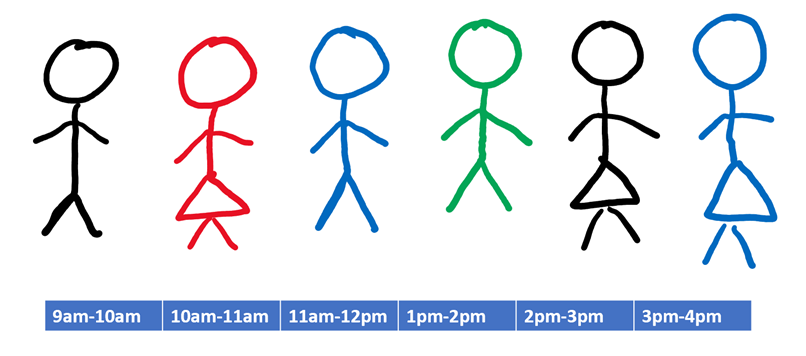
\includegraphics[keepaspectratio]{workers.png}}

}

\caption{Here is the alt text}

\end{figure}%

\paragraph*{Approach 2 (R)}\label{approach-2-r}
\addcontentsline{toc}{paragraph}{Approach 2 (R)}

This is a slightly more difficult approach and requires the use of R,
but it is better for ``hiding'' the alternative text.

\begin{Shaded}
\begin{Highlighting}[]
\InformationTok{\textasciigrave{}\textasciigrave{}\textasciigrave{}\{r, echo=FALSE, out.width="600px", fig.alt="Here is the alt text", fig.cap="Here is the image caption."\}}
\InformationTok{    knitr::include\_graphics("workers.png")}
\InformationTok{\textasciigrave{}\textasciigrave{}\textasciigrave{}}
\end{Highlighting}
\end{Shaded}

\begin{figure}[H]

{\centering 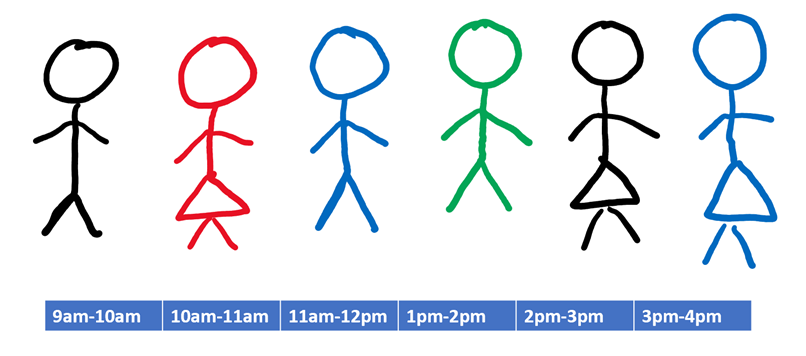
\includegraphics[width=6.25in,height=\textheight,keepaspectratio]{workers.png}

}

\caption{Here is the image caption.}

\end{figure}%

The student could view the alt text by right clicking on the image and
selecting ``Inspect Element'', or by using suitable assistive
technology.

This is the preferred approach since we can distinguish between image
captions and alt text. Also, we benefit from R's automatic numbering of
figures in their captions.

\subsubsection{Generating Images Using R (or
Python)}\label{generating-images-using-r-or-python}

Press Ctrl+Alt+I to add R code. This adds the chunk below and you can
add in R code. Python (or other languages) can also be added by pressing
the `+C' image at the top right corner.

\begin{Shaded}
\begin{Highlighting}[]
\NormalTok{x}\OtherTok{\textless{}{-}}\FunctionTok{rnorm}\NormalTok{(}\DecValTok{100}\NormalTok{,}\AttributeTok{mean=}\DecValTok{4}\NormalTok{,}\AttributeTok{sd=}\DecValTok{2}\NormalTok{)}
\NormalTok{y}\OtherTok{\textless{}{-}}\NormalTok{x}\SpecialCharTok{\^{}}\NormalTok{\{}\DecValTok{2}\NormalTok{\}}
\FunctionTok{plot}\NormalTok{(x,y,}\AttributeTok{lwd=}\DecValTok{4}\NormalTok{,}\AttributeTok{main=}\StringTok{"Mock plot"}\NormalTok{)}
\end{Highlighting}
\end{Shaded}

\begin{figure}[H]

{\centering \pandocbounded{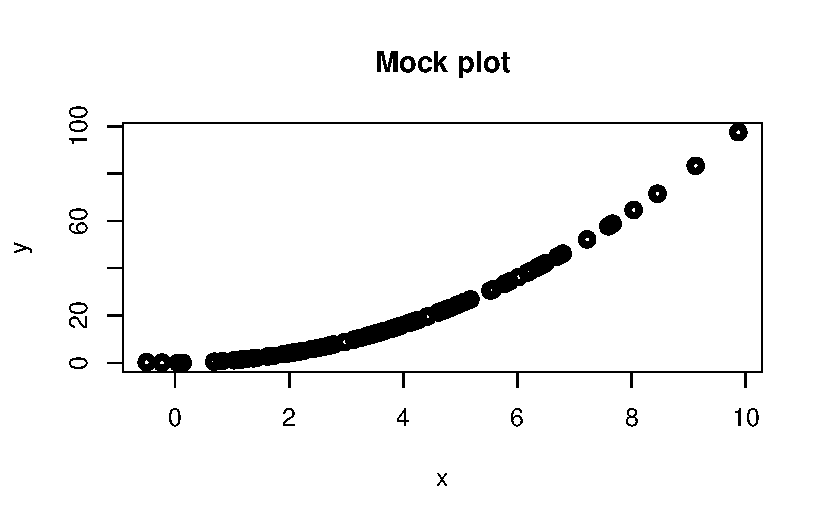
\includegraphics[keepaspectratio]{02-Part2_files/figure-pdf/unnamed-chunk-14-1.pdf}}

}

\caption{A graph demonstrating\ldots{}}

\end{figure}%

You can also hide code, so that graphs are produced without showing the
code, or you can hide output so the code is shown without the results
etc. see
\href{https://rstudio.com/wp-content/uploads/2015/02/rmarkdown-cheatsheet.pdf?target=_blank}{the
R Markdown cheatsheet} for more information.

The graph is produced but the code is hidden, by setting echo=FALSE.

\begin{figure}[H]

{\centering \pandocbounded{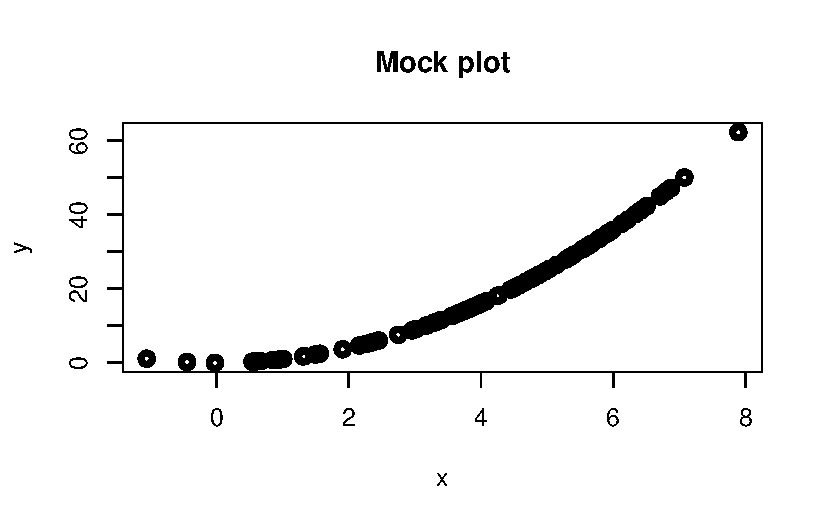
\includegraphics[keepaspectratio]{02-Part2_files/figure-pdf/unnamed-chunk-15-1.pdf}}

}

\caption{A graph demonstrating\ldots{}}

\end{figure}%

Here, the code is shown but the graph is not shown using eval=FALSE.

\begin{Shaded}
\begin{Highlighting}[]
\NormalTok{x}\OtherTok{\textless{}{-}}\FunctionTok{rnorm}\NormalTok{(}\DecValTok{100}\NormalTok{,}\AttributeTok{mean=}\DecValTok{4}\NormalTok{,}\AttributeTok{sd=}\DecValTok{2}\NormalTok{)}
\NormalTok{y}\OtherTok{\textless{}{-}}\NormalTok{x}\SpecialCharTok{\^{}}\NormalTok{\{}\DecValTok{2}\NormalTok{\}}
\FunctionTok{plot}\NormalTok{(x,y,}\AttributeTok{lwd=}\DecValTok{4}\NormalTok{,}\AttributeTok{main=}\StringTok{"Mock plot"}\NormalTok{)}
\end{Highlighting}
\end{Shaded}

\subsection{Environments}\label{environments}

R Bookdown has several built-in environments, such as Theorem, Example,
etc to help organise your notes.

\subsubsection{Numbered Environments}\label{numbered-environments}

The following environments have an automatic numbering system and so can
be cross-referenced.

\begin{longtable}[]{@{}lll@{}}
\caption{(\#tab:num-envs) Numbered Environments in R
Bookdown}\tabularnewline
\toprule\noalign{}
Environment & Printed Name & Label Prefix \\
\midrule\noalign{}
\endfirsthead
\toprule\noalign{}
Environment & Printed Name & Label Prefix \\
\midrule\noalign{}
\endhead
\bottomrule\noalign{}
\endlastfoot
theorem & Theorem & thm \\
lemma & Lemma & lem \\
corollary & Corollary & cor \\
proposition & Proposition & prp \\
conjecture & Conjecture & cnj \\
definition & Definition & def \\
example & Example & exm \\
exercise & Exercise & exr \\
hypothesis & Hypothesis & hyp \\
\end{longtable}

This green box is the \texttt{example} environment. To invoke the
\texttt{example} environment, use the syntax

\begin{Shaded}
\begin{Highlighting}[]
\NormalTok{::: \{.example name="Example Name"\}}
\NormalTok{\textless{}br\textgreater{}}
\NormalTok{Example text...}
\NormalTok{:::}
\end{Highlighting}
\end{Shaded}

If you do not wish to name your example, then write

\begin{Shaded}
\begin{Highlighting}[]
\NormalTok{:::example}
\NormalTok{\textless{}br\textgreater{}}
\NormalTok{Example text...}
\NormalTok{:::}
\end{Highlighting}
\end{Shaded}

The \texttt{\textless{}br\textgreater{}} tag is used to start the
example text on a new line.

\paragraph*{Cross Referencing
Environments}\label{cross-referencing-environments}
\addcontentsline{toc}{paragraph}{Cross Referencing Environments}

Numbered environments are cross referenced in a similar way to equations
(see \hyperref[mathematics]{Section 2.3}).

\begin{Shaded}
\begin{Highlighting}[]
\NormalTok{::: \{.theorem \#pyth name="Pythagoras\textquotesingle{} Theorem"\}}
\NormalTok{For a right triangle, if $c$ denotes the length of the hypotenuse}
\NormalTok{and $a$ and $b$ denote the lengths of the other two sides, we have}
\NormalTok{$$a\^{}2 + b\^{}2 = c\^{}2$$}
\NormalTok{:::}
  
\NormalTok{We use Pythagoras\textquotesingle{} Theorem \textbackslash{}@ref(thm:pyth) to find the length of the missing side.}
\end{Highlighting}
\end{Shaded}

\phantomsection\label{pyth}
For a right-angled triangle, if \(c\) denotes the length of the
hypotenuse and \(a\) and \(b\) denote the lengths of the other two
sides, we have \[a^2 + b^2 = c^2.\]

We use Pythagoras' Theorem @ref(thm:pyth) to find the length of the
missing side.

The syntax for referencing environments is
\texttt{\textbackslash{}@ref(\textless{}prefix\textgreater{}:\textless{}label\textgreater{})}.
Refer to Table @ref(tab:num-envs) for the prefix corresponding to each
environment type.

The prefix for a table reference is \texttt{tab}.

\subsubsection{Unnumbered Environments}\label{unnumbered-environments}

\begin{longtable}[]{@{}ll@{}}
\caption{(\#tab:oth-envs) Other Environments in R
Bookdown}\tabularnewline
\toprule\noalign{}
Environment & Printed Name \\
\midrule\noalign{}
\endfirsthead
\toprule\noalign{}
Environment & Printed Name \\
\midrule\noalign{}
\endhead
\bottomrule\noalign{}
\endlastfoot
proof & Proof \\
remark & Remark \\
note & Note \\
tip & Tip \\
activity & Activity \\
discussion & Discussion \\
solution & Solution \\
\end{longtable}

We have written a custom template for use in The School of Mathematical
Sciences with a specific colour scheme and some additional environments.
The code for the School Template is in \texttt{style.css}.

If you want to make adjustments to the colour scheme, or add your own
custom environments, then either edit your local copy of
\texttt{style.css}, or (if you're not familiar with CSS) contact
\href{mailto:tom.wicks@nottingham.ac.uk}{Tom} or
\href{mailto:lisa.mott@nottingham.ac.uk}{Lisa} to request a
change/update.

\bookmarksetup{startatroot}

\section{Interactivity}\label{interactivity}

The great thing with using HTML is that you can make your notes as
interactive as you like. This section shows you a few ways of
introducing interactivity to your notes, but the possibilities are
endless.

\subsection{Reveal Hidden Text}\label{reveal-hidden-text}

You can hide and unhide some text (e.g.~hints or optional solutions) as
in the following example.

Use the ``\textless details\textgreater{}'' and
``\textless summary\textgreater{}'' html tags to hide and reveal text
interactively.

\begin{Shaded}
\begin{Highlighting}[]
\DataTypeTok{\textless{}}\KeywordTok{details}\DataTypeTok{\textgreater{}}
  \DataTypeTok{\textless{}}\KeywordTok{summary}\DataTypeTok{\textgreater{}}\NormalTok{click to unhide}\DataTypeTok{\textless{}/}\KeywordTok{summary}\DataTypeTok{\textgreater{}}
\NormalTok{  Here is some hidden text.}
\DataTypeTok{\textless{}/}\KeywordTok{details}\DataTypeTok{\textgreater{}}
\end{Highlighting}
\end{Shaded}

click to unhide.

This is the text/image etc. that I want to hide.

\(a+b\)

\begin{Shaded}
\begin{Highlighting}[]
\NormalTok{x}\OtherTok{\textless{}{-}}\FunctionTok{rnorm}\NormalTok{(}\DecValTok{100}\NormalTok{,}\AttributeTok{mean=}\DecValTok{4}\NormalTok{,}\AttributeTok{sd=}\DecValTok{2}\NormalTok{)}
\NormalTok{y}\OtherTok{\textless{}{-}}\NormalTok{x}\SpecialCharTok{\^{}}\NormalTok{\{}\DecValTok{2}\NormalTok{\}}
\FunctionTok{plot}\NormalTok{(x,y,}\AttributeTok{lwd=}\DecValTok{4}\NormalTok{,}\AttributeTok{main=}\StringTok{"Mock plot"}\NormalTok{)}
\end{Highlighting}
\end{Shaded}

\begin{figure}[H]

{\centering \pandocbounded{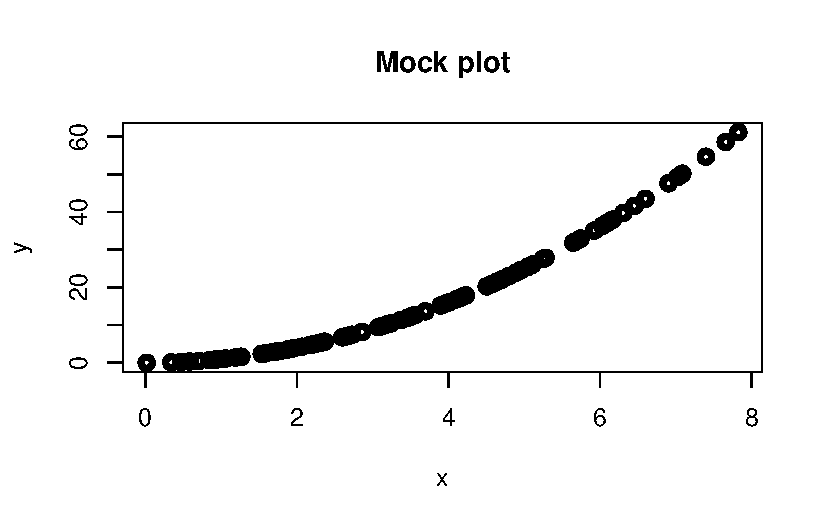
\includegraphics[keepaspectratio]{03-Part3_files/figure-pdf/unnamed-chunk-2-1.pdf}}

}

\caption{A graph demonstrating\ldots{}}

\end{figure}%

\subsection{Embedded Video}\label{embedded-video}

Please watch the video below to see how we have embedded this video from
mediaspace.

If the link does not work then please use
\href{https://mediaspace.nottingham.ac.uk/media/How+to+get+the+embed+links/1_824b1mfn}{this
alternative link.}

\textbf{How to use the template - Another video example}

Note to use all of this you will need R studio and R to be installed on
your machine. Then you just need to open the project in R studio.

Then in R studio just create a new .Rmd file to add a new chapter and
just save it as 01, 02, 03, 04 etc. in the name for the order you want
that chapter to appear.

A video below shows what to do in more detail. If the video does not
work then please use
\href{https://mediaspace.nottingham.ac.uk/media/How+to+use+the+template/1_brjfqb44}{this
alternative link.}

\subsection{Quizzes}\label{quizzes}

\subsubsection{Xerte}\label{xerte}

For Xerte, just paste the embed code. Example below. Note, if you have
your settings on Xerte so that the file can only be viewed from Moodle,
then the Xerte file will only show if the Rbookdown file is uploaded to
Moodle.

If the interactive slides above do not work then please access them
using \href{https://www.nottingham.ac.uk/toolkits/play_25775}{this
link.}

\subsubsection{Itempool}\label{itempool}

Here we use r commands to add in a URL.

\subsubsection{Microsoft Forms}\label{microsoft-forms}

This one has been used by copying and pasting the embed code from the
microsoft form share settings.

\bookmarksetup{startatroot}

\section{Adding colour}\label{adding-colour}

This is an advanced feature for bookdown and is not suitable for
beginners.

It is quite easy to use HTML to add {colour to text.} However when you
change the theme to night you will not be able to see the colour.

\href{https://www.nottingham.ac.uk/biosciences/people/qingqi.wang}{Steve
Wang} has provided a solution that uses HTML and R to use colours that
change in the three different themes.

In this template we have set three default colour schemes that are
accessible in all of the three themes.

If you would like to change the colour of some text you can do by
creating the following formula in R. The class myhl is defined in the
style file.

The below function is so you can see the output of the above function
and can be deleted.

\begin{Shaded}
\begin{Highlighting}[]
\NormalTok{colorize}\OtherTok{\textless{}{-}}\ControlFlowTok{function}\NormalTok{(x,color)\{}
  \ControlFlowTok{if}\NormalTok{ (knitr}\SpecialCharTok{::}\FunctionTok{is\_latex\_output}\NormalTok{()) \{}
    \FunctionTok{sprintf}\NormalTok{(}\StringTok{"}\SpecialCharTok{\textbackslash{}\textbackslash{}}\StringTok{textcolor\{\%s\}\{\%s\}"}\NormalTok{,color,x)}
\NormalTok{  \} }\ControlFlowTok{else} \ControlFlowTok{if}\NormalTok{ (knitr}\SpecialCharTok{::}\FunctionTok{is\_html\_output}\NormalTok{())\{}
    \FunctionTok{sprintf}\NormalTok{(}\StringTok{"\textless{}span class=\textquotesingle{}myhl\textquotesingle{}\textgreater{}\%s\textless{}/span\textgreater{}"}\NormalTok{ ,x)}
\NormalTok{  \} }\ControlFlowTok{else}\NormalTok{ x}
\NormalTok{\}}
\end{Highlighting}
\end{Shaded}

We can them add \textcolor{blue}{some words in blue.} You may want to
see what happens when you change the theme to night in the output.

We can then define another colour using the following

\begin{Shaded}
\begin{Highlighting}[]
\NormalTok{colorize2}\OtherTok{\textless{}{-}}\ControlFlowTok{function}\NormalTok{(x,color)\{}
  \ControlFlowTok{if}\NormalTok{ (knitr}\SpecialCharTok{::}\FunctionTok{is\_latex\_output}\NormalTok{()) \{}
    \FunctionTok{sprintf}\NormalTok{(}\StringTok{"}\SpecialCharTok{\textbackslash{}\textbackslash{}}\StringTok{textcolor\{\%s\}\{\%s\}"}\NormalTok{,color,x)}
\NormalTok{  \} }\ControlFlowTok{else} \ControlFlowTok{if}\NormalTok{ (knitr}\SpecialCharTok{::}\FunctionTok{is\_html\_output}\NormalTok{())\{}
    \FunctionTok{sprintf}\NormalTok{(}\StringTok{"\textless{}span class=\textquotesingle{}myhl2\textquotesingle{}\textgreater{}\%s\textless{}/span\textgreater{}"}\NormalTok{ ,x)}
\NormalTok{  \} }\ControlFlowTok{else}\NormalTok{ x}
\NormalTok{\}}
\end{Highlighting}
\end{Shaded}

Here is some text using the \textcolor{red}{red theme}

\begin{Shaded}
\begin{Highlighting}[]
\NormalTok{colorize3}\OtherTok{\textless{}{-}}\ControlFlowTok{function}\NormalTok{(x,color)\{}
  \ControlFlowTok{if}\NormalTok{ (knitr}\SpecialCharTok{::}\FunctionTok{is\_latex\_output}\NormalTok{()) \{}
    \FunctionTok{sprintf}\NormalTok{(}\StringTok{"}\SpecialCharTok{\textbackslash{}\textbackslash{}}\StringTok{textcolor\{\%s\}\{\%s\}"}\NormalTok{,color,x)}
\NormalTok{  \} }\ControlFlowTok{else} \ControlFlowTok{if}\NormalTok{ (knitr}\SpecialCharTok{::}\FunctionTok{is\_html\_output}\NormalTok{())\{}
    \FunctionTok{sprintf}\NormalTok{(}\StringTok{"\textless{}span class=\textquotesingle{}myhl3\textquotesingle{}\textgreater{}\%s\textless{}/span\textgreater{}"}\NormalTok{ ,x)}
\NormalTok{  \} }\ControlFlowTok{else}\NormalTok{ x}
\NormalTok{\}}
\end{Highlighting}
\end{Shaded}

Finally here is some text using the
\textcolor{green}{final colour scheme.}

\subsection{Adding colour to maths
output}\label{adding-colour-to-maths-output}

This is even more complicated and uses the style file. We have set three
default colours for blue, red and green that meet accessibility
requirements in the three different themes.

\[
g(\color{blue}{x-1}) = 3(\color{red}{x-1}) + 1 = \color{green}{3x} - 3 + 1 = 3x-2.
\]

\subsection{New box types}\label{new-box-types}

We have added some new box types to the template.

Watch out for this common mistake!

Here is a key point.




\end{document}
